% Shared preamble for the CAWASMA viva notes (Atta, Asim, Neelam).
\documentclass[11pt,a4paper]{article}
\usepackage[T1]{fontenc}
\usepackage[utf8]{inputenc}
\usepackage{lmodern}
\usepackage{amsmath}
\usepackage{amssymb}
\usepackage{microtype}
\usepackage[margin=2.3cm]{geometry}
\usepackage{booktabs}
\usepackage{array}
\usepackage{tabularx}
\usepackage{longtable}
\usepackage{xcolor}
\usepackage{enumitem}
\usepackage{caption}
\usepackage{listings}
\usepackage{tikz}
\usetikzlibrary{arrows.meta,positioning,fit,backgrounds,calc}
\usepackage[hidelinks]{hyperref}

\definecolor{brand}{HTML}{1F4E79}
\definecolor{soft}{HTML}{F3F6F9}
\definecolor{rule}{HTML}{B8C2CC}
\definecolor{codebg}{HTML}{F7F8FA}
\definecolor{kw}{HTML}{1F5FA8}
\definecolor{cm}{HTML}{6A7684}

\captionsetup{font=small,labelfont={bf,color=brand},justification=raggedright,singlelinecheck=false}
\setlist{itemsep=2pt,topsep=3pt,parsep=0pt}
\sloppy
\hbadness=6000
\renewcommand{\arraystretch}{1.18}

% Code excerpts: small, wrapping, no language assumptions.
\lstset{
  basicstyle=\ttfamily\footnotesize,
  backgroundcolor=\color{codebg},
  frame=single, rulecolor=\color{rule},
  breaklines=true, breakatwhitespace=false,
  keywordstyle=\color{kw}\bfseries,
  commentstyle=\color{cm}\itshape,
  showstringspaces=false,
  columns=fullflexible,
  xleftmargin=6pt, xrightmargin=6pt,
  aboveskip=6pt, belowskip=6pt,
  literate={->}{{$\rightarrow$}}1 {<-}{{$\leftarrow$}}1,
}
\lstdefinestyle{py}{language=Python}

% Source footnote: where a fact came from in the repo.
\newcommand{\src}[1]{\footnote{Source: \texttt{#1}}}

% Person title block. \setperson{Name}{Role}{Roll}
\newcommand{\PersonName}{} \newcommand{\PersonRole}{} \newcommand{\PersonRoll}{}
\newcommand{\setperson}[3]{\renewcommand{\PersonName}{#1}\renewcommand{\PersonRole}{#2}\renewcommand{\PersonRoll}{#3}}

\newcommand{\maketitlepage}{%
\begin{titlepage}
\centering
\vspace*{1.2cm}
{\color{brand}\rule{\linewidth}{1.2pt}}\\[4mm]
{\Large\bfseries CAWASMA}\\[2mm]
{\large Context-Aware Web \& API Security Misconfiguration Analyzer}\\[3mm]
{\color{brand}\rule{\linewidth}{1.2pt}}\\[1.4cm]
{\large Final-year project --- viva study notes}\\[1.2cm]
{\Huge\bfseries \PersonName}\\[5mm]
{\large \PersonRole}\\[3mm]
{\large Roll number: \PersonRoll}\\[1.4cm]
\begin{tabular}{rl}
Supervisor: & Dr.\ Bilal Khan\\[2mm]
Team: & Asim Shakeel (22P-9229)\\
 & Neelam Jabeen (22P-9353)\\
 & Atta Ur Rehman (22P-9236)\\
\end{tabular}\\[1.2cm]
{\color{cm}\small These notes are generated from the repository, documentation and git history.\\
Every number is cited to the file or command it came from. Date: \today.}\\[1cm]
{\color{brand}\rule{\linewidth}{0.6pt}}
\end{titlepage}}

% A small helper for the "scoring in one line" boxes.
\newcommand{\keybox}[1]{\par\vspace{3pt}\noindent\fcolorbox{rule}{soft}{\parbox{\dimexpr\linewidth-2\fboxsep-2\fboxrule}{#1}}\par\vspace{3pt}}

\setperson{Neelam Jabeen}{Frontend (Next.js web app)}{22P-9353}
\begin{document}
\maketitlepage
\tableofcontents
\clearpage

% Part A: the whole project. Shared, identical in all three documents.
\section{The whole project}

\subsection{The problem}
A normal security scanner gives a fixed severity to each kind of finding. A
missing \texttt{X-Content-Type-Options} header is ``medium'' wherever it is
found: on a public brochure page, and on a login API that returns credentials.
The person reading the report then has to work out, by hand, which of a hundred
``medium'' findings actually matters. That triage is slow and easy to get
wrong. Tools such as OWASP ZAP and Nuclei do find real issues, but they rate
the issue, not the place it sits in.\src{docs/supervisor/scanners.md}

\subsection{The idea}
CAWASMA scores the \emph{same} finding differently according to where it occurs
and what the endpoint returned. It does this with the standard CVSS v3.1
\emph{environmental} metrics, so the result is not an invented number: it is a
recomputation of the official score with a vector anyone can check on the FIRST
calculator.

\keybox{\textbf{One-paragraph pitch.} CAWASMA is a defensive, black-box,
HTTPS-only scanner for web apps and REST APIs. Each of its checks carries a
fixed CVSS v3.1 base vector. For every finding it works out how sensitive the
endpoint is (from the URL path) and what sensitive data the response holds
(credentials, personal data, financial data, internal IPs). It turns those into
CVSS environmental security requirements (CR/IR/AR) and recomputes the score, so
a login API and a public page that share a weakness no longer share a priority.
The point of the project is \emph{prioritisation, not detection}.}

\subsection{Architecture}
A scan is a pipeline. A URL goes in; a ranked, explained report comes out.

\begin{center}
\resizebox{0.98\linewidth}{!}{%
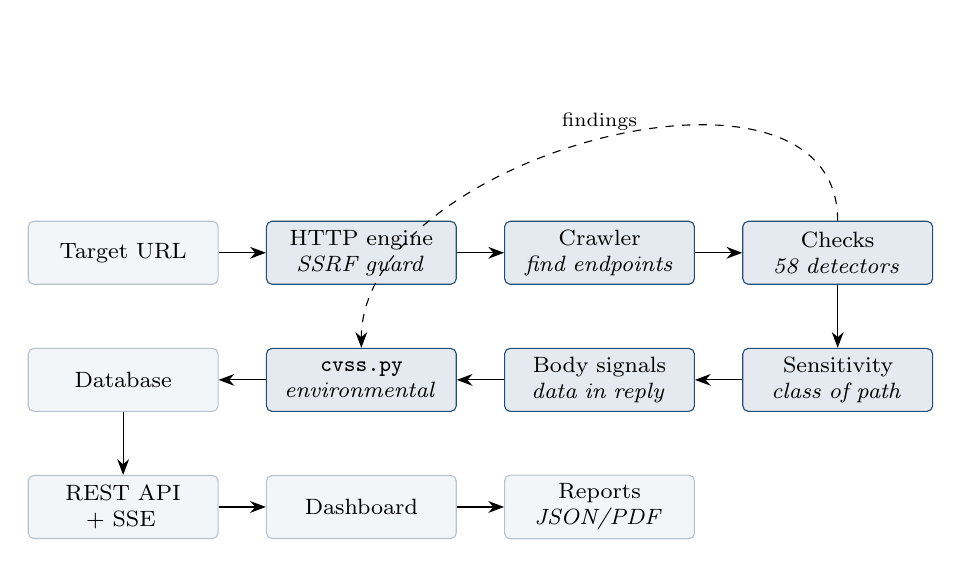
\begin{tikzpicture}[
  font=\footnotesize,
  >={Stealth[length=2mm]},
  box/.style={draw=rule,fill=soft,rounded corners=2pt,minimum height=8mm,inner sep=3pt,text width=22mm,align=center},
  core/.style={box,fill=brand!12,draw=brand},
  node distance=4mm and 6mm,
]
\node[box] (url) {Target URL};
\node[core,right=of url] (eng) {HTTP engine\\\textit{SSRF guard}};
\node[core,right=of eng] (crawl) {Crawler\\\textit{find endpoints}};
\node[core,right=of crawl] (checks) {Checks\\\textit{58 detectors}};
\node[core,below=8mm of checks] (sens) {Sensitivity\\\textit{class of path}};
\node[core,left=of sens] (body) {Body signals\\\textit{data in reply}};
\node[core,left=of body] (cvss) {\texttt{cvss.py}\\\textit{environmental}};
\node[box,left=of cvss] (db) {Database};
\node[box,below=8mm of db] (api) {REST API\\+ SSE};
\node[box,right=of api] (ui) {Dashboard};
\node[box,right=of ui] (rep) {Reports\\\textit{JSON/PDF}};
\draw[->] (url)--(eng); \draw[->] (eng)--(crawl); \draw[->] (crawl)--(checks);
\draw[->] (checks)--(sens); \draw[->] (sens)--(body); \draw[->] (body)--(cvss);
\draw[->] (cvss)--(db); \draw[->] (db)--(api); \draw[->] (api)--(ui); \draw[->] (ui)--(rep);
\draw[->,dashed] (checks.north) to[out=90,in=90] node[above,font=\scriptsize]{findings} (cvss.north);
\end{tikzpicture}}
\end{center}

\noindent The stages are: the \textbf{engine} fetches safely (one SSRF check per
redirect hop); the \textbf{crawler} discovers endpoints (seed, HTML, JavaScript,
a wordlist, and OpenAPI paths); the \textbf{checks} look for misconfigurations;
the \textbf{sensitivity} classifier labels each endpoint CRITICAL/HIGH/MEDIUM/LOW
from its path; the \textbf{body classifier} looks for sensitive data in the
reply; \texttt{cvss.py} turns those two into CR/IR/AR and recomputes the score;
the result is stored, served by the API over REST and Server-Sent Events, shown
on the dashboard, and exported as reports.

\subsection{Technology, and why}
\begin{center}
\small
\begin{tabularx}{\linewidth}{@{}p{34mm}X@{}}
\toprule
\textbf{Part} & \textbf{Choice and reason}\\
\midrule
Scanner core & Python 3.12 with \texttt{httpx} + \texttt{asyncio}: endpoints are analysed concurrently, and the core stays database-free so it is easy to test.\\
Scoring & The \texttt{cvss} library, so the environmental maths is the published CVSS v3.1 formula, not ours.\\
NLP & Sentence-Transformers (\texttt{all-MiniLM-L6-v2}) and spaCy for the sensitivity class; the engine still works with the built-in classifier when these are absent.\\
API & FastAPI, with Pydantic schemas and a frozen contract; Celery + Redis run scans in the background with live status.\\
Database & PostgreSQL in production, SQLite in tests; the models stay portable with a \texttt{JSONType} column and database-level cascades.\\
TLS & SSLyze (with a plain-\texttt{ssl} fallback) for the transport checks.\\
Reports & One HTML template through WeasyPrint for the PDF, so HTML and PDF never drift.\\
Frontend & Next.js 16 (App Router), React 19, TypeScript, Tailwind CSS v4, shadcn/ui, TanStack Query.\\
Tests & \texttt{pytest} (backend), Vitest + Testing Library and Playwright (frontend).\\
\bottomrule
\end{tabularx}
\end{center}

\subsection{Team roles and the shared contracts}
Three people own three areas, and they meet at three written contracts, frozen
so one person's change cannot silently break another's code.\src{CLAUDE.md; .github/CODEOWNERS}

\begin{center}
\small
\begin{tabularx}{\linewidth}{@{}p{24mm}X@{}}
\toprule
\textbf{Member} & \textbf{Owns}\\
\midrule
Asim (22P-9229) & Check specifications and their CVSS v3.1 vectors, the environmental mapping, chain templates, the sensitivity and response (ML/NLP) classifiers, and the whole evaluation lab.\\
Neelam (22P-9353) & The Next.js web app, the \texttt{frontend} service and its CI job.\\
Atta (22P-9236) & The backend: HTTP engine, crawler, check functions, CVSS scoring code, attack-chain engine, reports, FastAPI app, Celery workers, database and migrations, plus the shared infrastructure and reviews.\\
\bottomrule
\end{tabularx}
\end{center}

\begin{description}[leftmargin=0pt,itemsep=3pt]
\item[API contract (v1).] \texttt{app/api/schemas/contract.py} and
\texttt{docs/api-contract.md}: the field names the frontend reads
(\texttt{check\_id}, \texttt{base\_score}, \texttt{final\_score}, status
\texttt{DONE}).
\item[ML / CVSS contract.] \texttt{app/core/contracts.py} and
\texttt{docs/cvss-mapping-contract.md}: the types the engine and Asim's
classifiers exchange, so the engine keeps working with the built-in
classifiers when the ML packages are missing.
\item[Check-spec format.] \texttt{app/core/specs.py} and
\texttt{docs/check-spec-format.md}: how a check is declared so the registry can
run it.
\end{description}

\paragraph{Two scoring states.} Not every check is re-scored the new way yet.
Of 62 check ids, 25 have an approved specification and are scored through the
CVSS v3.1 environmental metrics; the other 37 still use an interim formula,
$\min(10,\ \text{base}\times\text{context multiplier}+\text{response bonus})$,
and each finding records which method scored it
(\texttt{scoring\_method}).\src{make coverage-stats; docs/06-scoring-model.md}

\clearpage

\section{What Neelam built}
Neelam owns the whole web app in \texttt{frontend/}: a Next.js 16 application
that starts a scan, shows it running live, and presents the ranked findings in a
way that \emph{explains} why each score moved. She also owns the \texttt{frontend}
Docker image, its compose service and its CI job.\src{.github/CODEOWNERS; CLAUDE.md}

\subsection{The typed API client}
\textbf{What it does.} \texttt{src/lib/api.ts} is the one place the app talks to
the backend. Every call returns an \texttt{ApiResult} and never throws, so each
screen handles success and failure the same way.

\textbf{How it works.} The functions are \texttt{createScan}, \texttt{getResults},
\texttt{getFindingDetail}, \texttt{cancelScan}, \texttt{listScans} and
\texttt{fetchExport}. Each resolves to \texttt{\{ok:true,data\}} or
\texttt{\{ok:false,error\}}, where the error is tagged \texttt{network},
\texttt{client} (4xx) or \texttt{server} (5xx). The contract types in
\texttt{api-types.ts} sit over \texttt{api-schema.ts}, which is generated from
\texttt{docs/openapi.json} and never hand-edited.

\begin{lstlisting}[caption={Errors are values, not exceptions (\texttt{src/lib/api.ts}).}]
export type ApiResult<T> =
  | { ok: true; data: T }
  | { ok: false; error: ApiError };   // network | client(4xx) | server(5xx)
\end{lstlisting}

\textbf{Design decision.} Returning results instead of throwing means no screen
can forget a \texttt{try/catch}; the type forces the error case to be handled.
\textbf{Inputs/outputs.} It consumes Atta's REST contract with the exact field
names (\texttt{check\_id}, \texttt{base\_score}, \texttt{final\_score}); nothing
is renamed on the client. \textbf{Tested by} \texttt{src/lib/api.test.ts}.
\textbf{Limitation:} the client mirrors the contract, so a contract change needs
a regenerated schema (\texttt{npm run gen:api}).

\subsection{Data fetching and live status}
\textbf{What it does.} Screens read data through TanStack Query hooks, and a
running scan updates itself live.

\textbf{How it works.} \texttt{queries.ts} has \texttt{useScanResults},
\texttt{useFindingDetail}, \texttt{useScanHistory}, \texttt{useCreateScan} and
\texttt{useCancelScan}. \texttt{use-live-scan.ts} follows the Server-Sent Events
stream \texttt{GET /api/scan/\{id\}/events}; if \texttt{EventSource} is missing or
the stream drops, it falls back to polling every two seconds. When the scan
reaches a terminal state the server ends the stream and the hook closes it so it
does not reconnect.

\textbf{Design decision.} SSE first, polling as a safety net, gives live updates
without a constant poll, and still works where SSE does not (the Next.js server
has no \texttt{EventSource}). \textbf{Tested by} \texttt{live-status.test.ts} and
the e2e flow. \textbf{Limitation:} the fallback poll adds up to two seconds of
lag when SSE is unavailable.

\subsection{New scan, ranked results, and explaining a score}
\textbf{What it does.} The home page starts a scan; the results page ranks the
findings and, for each one, tells the story of how its score changed.

\textbf{How it works.}
\begin{itemize}
\item \texttt{scan-form.ts} validates the URL and the ``I own this target''
confirmation before \texttt{createScan}; the backend enforces the same rules.
\item \texttt{findings-list.tsx} ranks by context-aware score, with a toggle to
``Base score''; \texttt{findings-filters.tsx} filters by severity, category,
OWASP and endpoint; \texttt{scan-summary.tsx} shows the severity counts and how
many findings moved up or down by context.
\item \texttt{finding-detail.tsx} with \texttt{score-story.ts} shows the base
score, the final score, the full CVSS vector with CR/IR/AR, the endpoint class
and the body signals --- the ``why this score'' story.
\end{itemize}

\begin{center}
\resizebox{0.98\linewidth}{!}{%
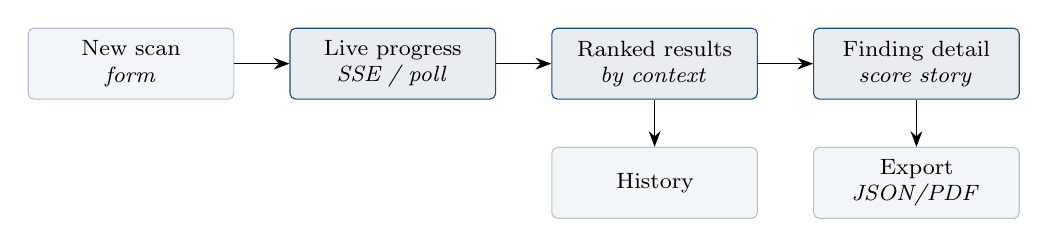
\begin{tikzpicture}[font=\footnotesize,>={Stealth[length=2mm]},
  s/.style={draw=rule,fill=soft,rounded corners=2pt,text width=24mm,align=center,minimum height=9mm,inner sep=3pt},
  d/.style={draw=brand,fill=brand!10},node distance=4mm and 7mm]
\node[s] (new){New scan\\\textit{form}};
\node[s,d,right=of new] (live){Live progress\\\textit{SSE / poll}};
\node[s,d,right=of live] (res){Ranked results\\\textit{by context}};
\node[s,d,right=of res] (det){Finding detail\\\textit{score story}};
\node[s,below=6mm of res] (hist){History};
\node[s,below=6mm of det] (exp){Export\\\textit{JSON/PDF}};
\draw[->](new)--(live);\draw[->](live)--(res);\draw[->](res)--(det);
\draw[->](res)--(hist);\draw[->](det)--(exp);
\end{tikzpicture}}
\end{center}

\textbf{Design decision.} The UI never recomputes a score; it shows the base and
final numbers the backend produced and explains them, so the app and the report
always agree. \textbf{Tested by} component tests and the e2e flows.
\textbf{Limitation:} very large scans are paged; the UI shows up to a few hundred
findings at once.

\subsection{Live progress, history and the evaluation page}
\textbf{What it does.} \texttt{live-progress.tsx} shows stages, elapsed time and
counts while a scan runs; \texttt{scan-history.tsx} lists past scans with
re-scan; the Evaluation page charts the project's own results.

\textbf{How it works.} The Evaluation page reads the final CSVs
(\texttt{eval/results/final/}) through \texttt{src/data/evaluation.json}, synced
by \texttt{npm run sync:eval}. Its charts are \texttt{confusion-matrix.tsx},
\texttt{ranking-compare.tsx} and \texttt{grouped-bars.tsx}.
\textbf{Design decision.} The numbers are built in at build time from the
evaluation output, so the page cannot drift from the harness.
\textbf{Limitation:} refreshing the page's numbers needs a re-sync and rebuild.

\subsection{Mock mode and the Docker/CI setup}
\textbf{What it does.} The app runs with no backend using MSW mocks, and ships as
a small standalone Docker image with its own CI job.

\textbf{How it works.} \texttt{src/mocks/} serves fixtures copied from
\texttt{docs/examples/} (a test fails if they drift), a simulated scan that goes
QUEUED $\rightarrow$ RUNNING $\rightarrow$ DONE in about ten seconds with its own
SSE stream and cancel, and a 600-finding scan for performance. The
\texttt{Dockerfile} builds an \texttt{output: "standalone"} server running as a
non-root user; the \texttt{frontend} CI job runs lint, format, typecheck, unit
tests, build and Playwright.
\textbf{Design decision.} \texttt{NEXT\_PUBLIC\_USE\_MOCK} makes every API call
come from fixtures, so the UI can be developed and demoed with no backend.
\textbf{Limitation:} mock mode mirrors the fixtures, so a new backend field needs
the fixtures updated too.

\section{Numbers to know}
All figures are from the repository at commit \texttt{7cc819f}.

\subsection{Tests the frontend carries}
\begin{center}\small
\begin{tabularx}{\linewidth}{@{}lX@{}}
\toprule
Suite & What it proves\\
\midrule
25 unit test files (Vitest) & The API client, hooks, score story, filters, formatting.\src{git ls-files}\\
\texttt{a11y.spec.ts} & No axe accessibility violations on the main pages.\\
\texttt{performance.spec.ts} & The 600-finding scan renders within budget.\\
\texttt{definition-of-done.spec.ts} & The seven definition-of-done items pass end to end.\\
\texttt{eval-flow.spec.ts}, \texttt{real-stack.spec.ts} & The full flow against the real backend.\\
\texttt{home.spec.ts}, \texttt{demo/demo.spec.ts} & The new-scan page and the demo recording.\\
\bottomrule
\end{tabularx}
\end{center}

\subsection{What the UI shows}
The Evaluation page presents the project's headline numbers: detection recall
(CAWASMA 0.758, Nuclei 0.765, ZAP 0.333, all precision
1.00)\src{eval/results/final/tools.md} and the base-vs-context ranking (mean
NDCG@10 $0.324\rightarrow0.347$).\src{eval/results/final/ranking\_environmental.md}
The results page shows, per scan, how many findings moved up or down a severity
because of context.

\section{Contribution timeline}
Grouped from merged pull requests.\src{gh pr list (upstream); git log}
\begin{center}\small
\begin{tabularx}{\linewidth}{@{}llX@{}}
\toprule
Merged & PRs & What changed\\
\midrule
24 Oct & \#6 & Frontend project setup (Next.js, Tailwind, shadcn).\\
26 Oct & \#29 & Typed API client and contract types.\\
26 Oct & \#30, \#31 & App shell; restore the shell lost in a merge.\\
26 Oct & \#32 & The new-scan page.\\
26 Oct & \#33, \#35 & Scan results and the results view.\\
26 Oct & \#34 & End-to-end tests against the real stack.\\
4 Nov & \#41, \#42 & Contract version 1.2; the finding-detail page with the score story.\\
4 Nov & \#43 & Live SSE status.\\
4 Nov & \#44 & Scan history.\\
4 Nov & \#50, \#51 & Export polish; the evaluation demo page.\\
\bottomrule
\end{tabularx}
\end{center}
\textbf{Reviews received.} Atta pushed fixes inside \texttt{frontend/} on
\texttt{atta/fix-neelam-*} branches for Neelam to review: API-schema sync
(\#54), fixture refreshes (\#59, \#64, \#66), security headers (\#63),
responsive fixes (\#73) and an unused export (\#75).

\section{Viva preparation}
\subsection{Likely questions, with short answers}
\begin{enumerate}[leftmargin=*,itemsep=3pt]
\item \textbf{Server or Client Components --- how do you decide?} Server
Components by default; \texttt{"use client"} only where there is interactivity,
such as the live scan and the filters.
\item \textbf{How does the UI show a scan running live?} \texttt{use-live-scan.ts}
subscribes to the SSE stream and falls back to a two-second poll if SSE is
unavailable or drops.
\item \textbf{Why both SSE and polling?} SSE gives push updates without constant
requests; polling is the safety net, including on the Next.js server which has no
\texttt{EventSource}.
\item \textbf{How does the client avoid crashing on an API error?} Every call
returns an \texttt{ApiResult}; the type forces each screen to handle the error
case, so nothing throws.
\item \textbf{How does the UI explain a score?} \texttt{finding-detail.tsx} with
\texttt{score-story.ts} shows base score, final score, the CVSS vector with
CR/IR/AR, the endpoint class and the body signals.
\item \textbf{Does the client ever compute a score?} No. It only displays the
base and final numbers the backend produced, so the app and the PDF agree.
\item \textbf{Why generate the API types?} \texttt{api-schema.ts} comes from
\texttt{docs/openapi.json} (\texttt{npm run gen:api}); the contract is the single
source of truth and the client cannot drift from it.
\item \textbf{How can you develop with no backend?} \texttt{NEXT\_PUBLIC\_USE\_MOCK}
serves every call from MSW fixtures, including a simulated scan with its own SSE
stream.
\item \textbf{How do you keep the mocks honest?} The fixtures are copied from
\texttt{docs/examples/}, and a test fails if they drift from the backend's
examples.
\item \textbf{How do you test accessibility?} \texttt{a11y.spec.ts} runs axe on
the main pages and fails on any violation.
\item \textbf{How does the UI cope with 600 findings?}
\texttt{performance.spec.ts} checks the 600-finding scan renders within budget;
the list is filtered and paged.
\item \textbf{What is Next.js 16 specific here?} The App Router with a
\texttt{src/} directory, Server Components, and APIs that differ from older
Next.js, so the team checks the bundled Next docs before relying on memory.
\item \textbf{How is the app shipped?} A multi-stage \texttt{Dockerfile} with
\texttt{output: "standalone"}, run as a non-root user; a separate CI job runs
lint, types, unit tests, build and Playwright.
\item \textbf{How does the browser reach the API in Docker?}
\texttt{NEXT\_PUBLIC\_API\_URL} is the browser URL (build-time);
\texttt{API\_INTERNAL\_URL} is the server-side URL (runtime,
\texttt{http://api:8000}).
\item \textbf{How does the results page show the project's point?} The summary
shows how many findings moved up or down a severity because of context, next to
the severity counts.
\item \textbf{How does the Evaluation page get its numbers?} From
\texttt{src/data/evaluation.json}, synced from \texttt{eval/results/final/} at
build time, so it matches the harness.
\item \textbf{What happens when a scan is cancelled from the UI?}
\texttt{useCancelScan} calls \texttt{cancelScan}; the backend sets the cancel
flag and the live stream shows the scan stop.
\item \textbf{Why TanStack Query?} It caches and revalidates server state, so the
screens stay in sync without hand-written fetching logic.
\item \textbf{How do you keep styling consistent?} Tailwind CSS v4 with shadcn/ui
components added through its CLI.
\item \textbf{What is the biggest UI limitation?} Very large scans are paged, and
the Evaluation page needs a re-sync and rebuild to update its numbers.
\item \textbf{How do you stop the API types drifting from the backend?} They are
generated from \texttt{docs/openapi.json}, and a test checks the fixtures against
the backend's examples, so a mismatch fails CI.
\item \textbf{What does the finding-detail page let the user verify?} It links to
the FIRST CVSS calculator for both the base and the environmental score, and
shows the OWASP and CWE standards for the check.
\item \textbf{Why can the SSE mock only run in some places?} \texttt{EventSource}
exists in the browser and in tests but not on the Next.js server, so the mock's
\texttt{sse()} is registered only where it exists.
\item \textbf{How is CORS handled between the app and the API?} The API's
allow-list (\texttt{FRONTEND\_ORIGIN}) defaults to the app's origin
(\texttt{localhost:3000}); if the app is served elsewhere, both change together.
\item \textbf{Why keep the lockfile npm-10 compatible?} Node 22 ships npm 10;
installing with npm 11 must be followed by \texttt{npx npm@10 install}, or
\texttt{npm ci} fails in Docker and CI.
\item \textbf{How does the results page make the project's point obvious?} The
summary shows how many findings moved up or down a severity because of context,
right next to the plain severity counts.
\item \textbf{What runs in the frontend CI job?} Lint, format check, typecheck,
unit tests, the production build, and Playwright --- plus a separate job that runs
the full flow against the real backend.
\end{enumerate}

\subsection{Three-minute demo script}
\begin{enumerate}[leftmargin=*]
\item Open the home page. Fill a target, tick ``I own this target'', start a scan.
\item Watch the live progress. Say: ``This is the SSE stream; it falls back to a
two-second poll.''
\item Open the ranked results. Toggle ``Base score'' and back. Say: ``Context
re-ranks the list; the base order is one click away.''
\item Open a finding. Walk through base $\rightarrow$ final, the CVSS vector, the
endpoint class and the body signals.
\item Export the PDF, then open the History and Evaluation pages.
\end{enumerate}

\subsection{Five things to explain without notes}
\begin{enumerate}[leftmargin=*]
\item The \texttt{ApiResult} pattern: errors are values, every screen handles
them.
\item Live status: SSE first, two-second poll as a fallback.
\item The finding-detail score story: base, final, vector, class, signals.
\item The app never recomputes a score; it displays and explains the backend's.
\item Mock mode and how the fixtures are kept honest.
\end{enumerate}

% Part F: glossary. Shared, identical in all three documents.
\section{Glossary}
\begin{description}[leftmargin=0pt,style=nextline,itemsep=3pt]
\item[CVSS base score] The standard severity of a vulnerability on its own, 0--10,
from a vector such as \texttt{AV:N/AC:L/\dots}. Fixed per check; never invented per scan.
\item[CVSS environmental score] The base score recomputed for a particular
environment, using CR/IR/AR and modified base metrics. CAWASMA's context-aware
score is this.
\item[CR / IR / AR] Confidentiality, Integrity and Availability \emph{Requirements}:
environmental inputs saying how much each property matters here. Values Low,
Medium, High, or X (Not Defined). CAWASMA sets them from the endpoint class and
the data in the response.
\item[Sensitivity class] CAWASMA's label for how sensitive an endpoint is ---
CRITICAL, HIGH, MEDIUM or LOW --- from the words in its URL path.
\item[Body signals] Sensitive data found in a response: credentials, personal
data (PII), financial data, or an internal IP address. Evidence is redacted.
\item[Base vs.\ final score] CAWASMA always keeps both: the official base score
and the context-aware (environmental) final score, in separate columns.
\item[Legacy vs.\ environmental scoring] A finding is scored either by the CVSS
environmental metrics (approved specs) or by the interim legacy formula; its
\texttt{scoring\_method} says which.
\item[Precision] Of the findings that were judged, the fraction that were
correct: $\text{TP}/(\text{TP}+\text{FP})$.
\item[Recall] Of the real issues in the answer key, the fraction found:
$\text{TP}/(\text{TP}+\text{FN})$.
\item[FPR] False-positive rate: $\text{FP}/(\text{FP}+\text{TN})$.
\item[Ground truth] A hand-written list, per target, of which check should
(\texttt{present}) or should not (\texttt{absent}) fire on which endpoint.
\item[NDCG@10] Normalised Discounted Cumulative Gain at rank 10: a score for how
well a ranking puts the important items near the top, against a graded list.
\item[Tie-break sampling] Base scores tie often, so a ranking's NDCG is averaged
over 1000 random orderings of the tied items, with a fixed seed.
\item[SSRF] Server-Side Request Forgery: tricking the scanner into requesting an
internal address. CAWASMA guards against it by validating the resolved IP on
every hop.
\item[Soft-404] A page that returns HTTP 200 but is really ``not found''. The
crawler learns a baseline so it does not treat these as real endpoints.
\item[Passive vs.\ active scan] Passive sends only safe GET/HEAD and reads what
comes back; active sends extra, still non-destructive, probes. CAWASMA never
sends attack payloads.
\item[BOLA / IDOR] Broken Object-Level Authorisation / Insecure Direct Object
Reference: reading another user's object by changing an id. CAWASMA only flags an
\emph{indicator}; confirming it needs logged-in accounts, which is future work.
\item[Attack chain] Several findings that together make a bigger risk, correlated
from a template and scored with their own composite vector.
\item[Environmental metric ``X''] ``Not Defined'': the neutral baseline. A public
(LOW) endpoint uses X, so its score is unchanged --- context only ever raises a
score here, it does not lower a public page below its base.
\end{description}

\end{document}
